% !TeX spellcheck = en_US
\documentclass[12pt]{article}
\usepackage[unicode=true]{hyperref}
\usepackage[utf8x]{inputenc}
\usepackage{amsmath,amsthm,amsfonts,eucal}
\usepackage{graphicx}

\title{Applications of the Fresnel Integrals}
\author{Jack Jones}
\date{March 17\th, 2019}


\newcommand\defbb[2]{\def#1{{\mathbb{#2}}}}
\newcommand\defbf[2]{\def#1{{\mathbf{#2}}}}
\newcommand\defcal[2]{\def#1{{\mathcal{#2}}}} % capital letters only
\newcommand\defrm[2]{\def#1{{\mathrm{#2}}}}
\newcommand\defsf[2]{\def#1{{\mathsf{#2}}}}
\newcommand\defvec[2]{\def#1{{\vec{#2}}}}
\def\vec{\mathbf}
\renewcommand\th[1][th]{$^{\text{#1}}$}
\newtheorem{thm}{T`heorem}

%\let\C=\relax
\DeclareMathOperator\Cee{C} % C(x) := \int_0^x cos(t^2) \d{t}
\defbb\CC{C} % complex numbers
\defrm\ud{d}
\def\d#1{{\,\ud#1\,}}
\newcommand\udfrac[2]{\ensuremath{\frac{\ud#1}{\ud #2}}}
\defrm\e{e}  % Euler's number
\DeclareMathOperator\erf{erf} % error function
\defsf\si{i} % \sqrt{-1}
\defbb\R{R}
%\let\S=\relax
\DeclareMathOperator\eS{S} % S(x) :=int_0^x sin(t^2) \d{t}


\begin{document}
\maketitle
\begin{abstract}

The Euler spiral, defined by the linear relationship between curvature and arc length, is a beautiful and elegant plane curve. Its underlying mathematical equation is most
commonly known as the Fresnel integrals. However, the Fresnel integrals and Euler spiral are  two views of one and the same thing. In this paper, we focus on Fresnel integral and study its properties and useful applications. In optics, the illumination
intensity at a point behind a slit is computed from
the distance between two points on the Euler spiral. The Euler spiral also provides optimal curvature for train tracks between a straight run and
an upcoming bend


\end{abstract}
\clearpage


\section{Introduction}
An Euler spiral is a curve whose curvature changes linearly with its curve length. Taking the example of peeling an orange with a kitchen knife, one can either cut the skin along meridians, or cut it along a spiral as the left image in Figure~\ref{f:orangePeel} shows. The red lines marked on the orange refer to the route one can follow to peel the orange. Later, if we unfold the spiral strip and flatten it on a table, we will see a long curve which is curved differently at different positions. Imagine that we will now cut the peel with progressively thinner strip widths, what we will obtain in the end is a long beautiful curve known as Euler spiral, as the left-side image in Figure~\ref{f:orangePeel} shows. According to Alfred Gray, Euler spiral is “one of the most elegant of all plane curves.” \cite{ASG17}


\begin{figure}[h!]
	\centering
	\includegraphics[height=5cm]{orange.jpg} \hfill
	\includegraphics[height=5cm]{orangePeel.jpg}
	\label{f:orangePeel}
	\caption{Left: Peeling an orange in a spiral of height $1/N$.
		Right: The flattened orange peel that resembles an Euler spiral.  Photos taken from \cite{BH12}.
	}
\end{figure}

For a mathematician, an interesting question is whether there are any equations that can describe the corresponding shape of an Euler spiral. For this we consider the Fresnel integrals.  These are defined as integrals over some elementary functions which can however not be integrated in elementary functions.  These integrals occur naturally in the description of the optics of an illuminated slit (in Subsection~\ref{s:relation}).


\subsection{Definition of Euler Spiral}
The Euler Spiral is defined by the  linear relationship between curvature and arc length, was
first proposed as a problem of elasticity by James Bernoulli, then solved accurately by Leonhard Euler \cite{Lev08}.
The Euler spiral is a curve in the complex plane that has curvature proportional to the arc length.  Here the arc length $s(t)$ of a differentiable curve $(x(t),y(t))$ in the plane is defined by
\[  \left(\udfrac{s}{t}\right)^2 := \left(\udfrac{x}{t}\right)^2 +\left(\udfrac{y}{t}\right)^2.
\]  Note that the curve length is monotone increasing with the parameter $t$ of the curve.  For a nice curve, it is possible to rewrite the curve in the arc length, i.e.~$(x(s),y(s))$.

The curvature of a smooth curve $\kappa$ can be defined as 
\[  \kappa=\frac1R = x'y'' -x''y'
\] if we assume that the curve is parameterized in the arc length $s$ \cite{BH12}.

According to \cite{BH12} the peel of the orange can be approximated as:
\begin{equation}
  \kappa \sim s  \label{e:eulerSpiral}
\end{equation}

The question we want to answer is how to describe the solution of this differential equation explicitly.  Therefore we introduce the Fresnel integrals.


\subsection{Definition of the Fresnel Integrals}
The Fresnel sine and cosine integrals are represented by  $S(x)$ and $C(x)$, which are two integral functions that originate by applying the analysis of Fresnel diffraction phenomena. The mathematical equations are as follows:

\begin{align}
\eS(x) &:= \int_0^x  \sin\left(\frac\pi2 t^2\right) \d{t}, \\
\Cee(x) &:= \int_0^x \cos\left(\frac\pi2 t^2\right) \d{t},
\end{align}
where $x \ge 0$ is a real number and $t$ is a real variable. When x tends to infinite, $S=C=1/2$.

The difficulty is that these integrals cannot be computed with analytic means, i.e.~the functions are transcendental \cite[p.195ff]{AS}.  This is in contrast to, e.g.
$$ \int_0^x (\sin t)^2 \d{t} = \frac12\int_0^x \left(1-\cos(2t)\right)\d{t} = \frac12x -\frac14\sin(2x).
$$


\subsection{Mathematical history}
The Fresnel integral and the related Euler spiral were discovered multiple times during history.  One of the first occurrances is according to \cite{Lev08} by J. Bernoulli in 1694 where he defines a curve such that an ideal metal rod of this shape unwinds to a straight line when placed under load at the ends.  In 1744, Euler is able to describe the curve by a differential equation that also allows him to reformulate it as the Fresnel integral.  37 years later he is able to compute the limiting points ($t\to\pm\infty$) of the curve and integrals.  Fresnel rediscovers the curve in 1818 and successfully applies it to the diffraction on a slit \cite{Lev08}.  He is also able to compute a couple of values numerically.  In 1874 Cornu plotted the curve accurately and proposes it as a graphical means for computing diffraction problems.

In the following sections, we will first describe the important properties of the Fresnel integrals followed by some important applications of it.

\section{Properties of the Fresnel Integrals}
\subsection{Basic properties}
The Fresnel integrals are odd, i.e.
\begin{align*}
	\eS(-x) &= \eS(x), & \Cee(-x) &= \Cee(x).
\end{align*}
\begin{proof}[Idea of proof]  The integrands $\sin(t^2)$ and $\cos(t^2)$ are even in $t$ and an anti-derivative $F(x)$ of an even function is odd if in addition $F(0)=0$.  The latter follows, because both integrals start at $t=0$.
\end{proof}

Their limits are
\[  \lim_{x\to\infty} \eS(x) = 0.5\sqrt{\tfrac\pi2},\qquad  \lim_{x\to\infty} \Cee(x) = 0.5\sqrt{\tfrac\pi2}.
\]

Since the integrals cannot be computed by elementary analytic means, an alternative is to compute them with a power series.  Therefore we present the Taylor expansion as
\begin{align*}
  \eS(x) &= \sqrt{\frac\pi2}\sum_{n\ge0} (-1)^nx^{4n+3}\frac{(\pi/2)^{2n+1}}{(2n+1)!(4n+3)}, \\
  \Cee(x) &= \sqrt{\frac\pi2}\sum_{n\ge0} (-1)^nx^{4n+1}\frac{(\pi/2)^{2n}}{(2n)!(4n+1)}.
\end{align*}
\begin{proof}[Idea of proof]  Start from the well known Taylor expansion of $\sin t = \sum_{n\ge0}$ $(-1)^n t^{2n+1}/(2n+1)!$ and $\cos t = \sum_{n\ge0} (-1)^nt^{2n}/(2n)!$, substitute $t\mapsto \tfrac\pi2 t^2$ and take the antiderivative for each summand.  The resulting series are $\eS(t)$ and $\Cee(t)$, because the integral of an absolutely converging power series equals the absolutely converging power series of the integrals of the summands.
\end{proof}

\begin{figure}[h!]
	\centering
	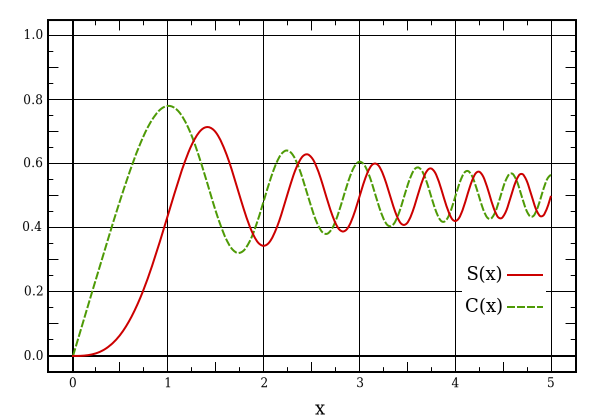
\includegraphics[width=0.5\textwidth]{Fresnel-Integrals-(Normalised).png}
	\caption{Fresnel integrals \cite{wiki}.}
\end{figure}

\subsection{Relation to the Euler spiral}\label{s:relation}
\begin{thm}  The curve $(x,y)=(C(t),S(t))$ is an Euler spiral.
\end{thm}
\begin{proof}  Let us start with showing that $t$ is the parameter of the arc length.  Consider therefore the derivatives
\begin{align*}
  C'(t) &= \frac\pi2\cos\left(\frac\pi2 t^2\right), &  
  S'(t) &= \frac\pi2\sin\left(\frac\pi2 t^2\right), \\
  C''(t) &= -\left(\frac\pi2\right)^2\sin\left(\frac\pi2 t^2\right)\cdot 2t, &
  S''(t) ^= \left(\frac\pi2\right)^2\cos\left(\frac\pi2 t^2\right)\cdot 2t.
\intertext{Then}
  \left(\udfrac{s}{t}\right)^2 &= \left(\frac\pi2\right)^2 \sim t
\end{align*}
I.e.~up to a constant factor $t$ is the arc length of the curve.

Let us now consider the curvature
\begin{align*}
  \kappa &= x'y''-x''y' \sim C'(t)S''(t)-C''(t)S'(t) = \frac{\pi}{2}2t \sim t
\end{align*}
\end{proof}

\begin{figure}[h!]
	\centering
	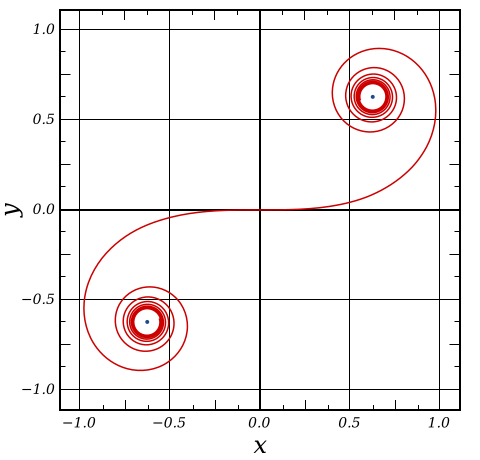
\includegraphics[width=0.5\textwidth]{eulerSpiral.png}
	\label{f:eulerSpiral}
	\caption{Euler spiral $(x,y)=(\Cee(t),\eS(t))$ \cite{wiki}.}
\end{figure}


\subsection{Other expressions}
The Fresnel integrals are closely related to the error function which is defined as follows
$$  \erf(x) := \int_{-x}^x \exp(-t^2) \d{t}.
$$
Also this function is analytic and can therefore be expanded to the whole complex plane.  Here the integral for fixed endpoints is independent of the path.

Now for the complex definition of exponential function
\begin{align*}  \exp(x+\si y) &:= (\cos y +\si\sin y)\e^x
\intertext{we obtain}
  \Cee(z)+\si\eS(z) &= \int_0^z \exp\left(\si\frac\pi2 t^2\right)\d{t} 
\intertext{Now we do a substitution in the complex plane as $t'=\sqrt{i}t$, i.e.~$\d{t'}=\frac{1+\si}{\sqrt{2}}\d{t}$ and obtain}
  &= \frac{1-\si}{\sqrt{2}}\int_0^{\frac{1+\si}{\sqrt{2}}} \exp(t^{\prime2}) \d{t'} = \frac12\,\frac{1-\si}{\sqrt2} \erf\left(\frac{1+\si}{\sqrt2}\,\frac\pi2 z\right).
\end{align*}
Therefore we can say that the Fresnel integrals are the real and imaginary part of the complex error function.


\section{Applications of Fresnel Integral}

The error functions, Fresnel integrals, and related functions occur in a variety of physical applications. Fresnel integrals and Cornu’s spiral occurred originally in the analysis of the diffraction of light; see Born and Wolf (1999, §8.7). More recently, Cornu’s spiral appears in the design of highways and railroad tracks, robot trajectory planning, and computer-aided design; see Meek and Walton (1992).

In optics, the illumination intensity at a point behind a slit is computed from the distance between two points on the Euler spi- ral. The Euler spiral also provides optimal curva- ture for train tracks between a straight run and an upcoming bend. It is striking that it can be also obtained with an orange and a kitchen knife.

The Euler spiral has applications in many fields of science. 

The Euler spiral has applications in
many fields of science. In optics, the illumination
intensity at a point behind a slit is computed from
the distance between two points on the Euler spiral. The Euler spiral also provides optimal curvature for train tracks between a straight run and
an upcoming bend. 

Fraunhofer diffraction, asymptotics of Weyl sums, and railway and freeway constructions.


\subsection{Application using the Euler Spiral}
\cite{BH12}
Electromagnetic field intensity
 in the physics of diffraction and is used in the theory of driving motorcar round a corner quickly.
 
\subsection{Further Applications}


\section{Conclusion}

\bibliographystyle{alphasorteprint}
\bibliography{bibliography.bib}
\nocite{AS, BE, Sim, Str, WW}  % TODO: place in text
\end{document}
